\chapter{Appendix: In-depth flight analysis}
\label{sec:specific_runs}

In the following, a detailed flight log is shown for the test setting of spawning at a fixed location on the Arroyo map and flying a random mission at 100 m altitude.

This example shows an ordinary flight where the drone took off from the ground, flew to a mission way point at cruise altitude and attempted to land twice which the second attempt was successful.

\subsection{Landing position}

As for \cref{chapter:evaluation}, the landing attempts are shown in \cref{fig:demo_run_landing}.


The mission way point in this run was quite close to the center. Therefore, it comes to no surprise that a landing site at the start plateau was chosen. One landing site was chosen but not verified and a close by site was subsequently chosen.

\clearpage%HERE

\begin{figure}[h]
\centering
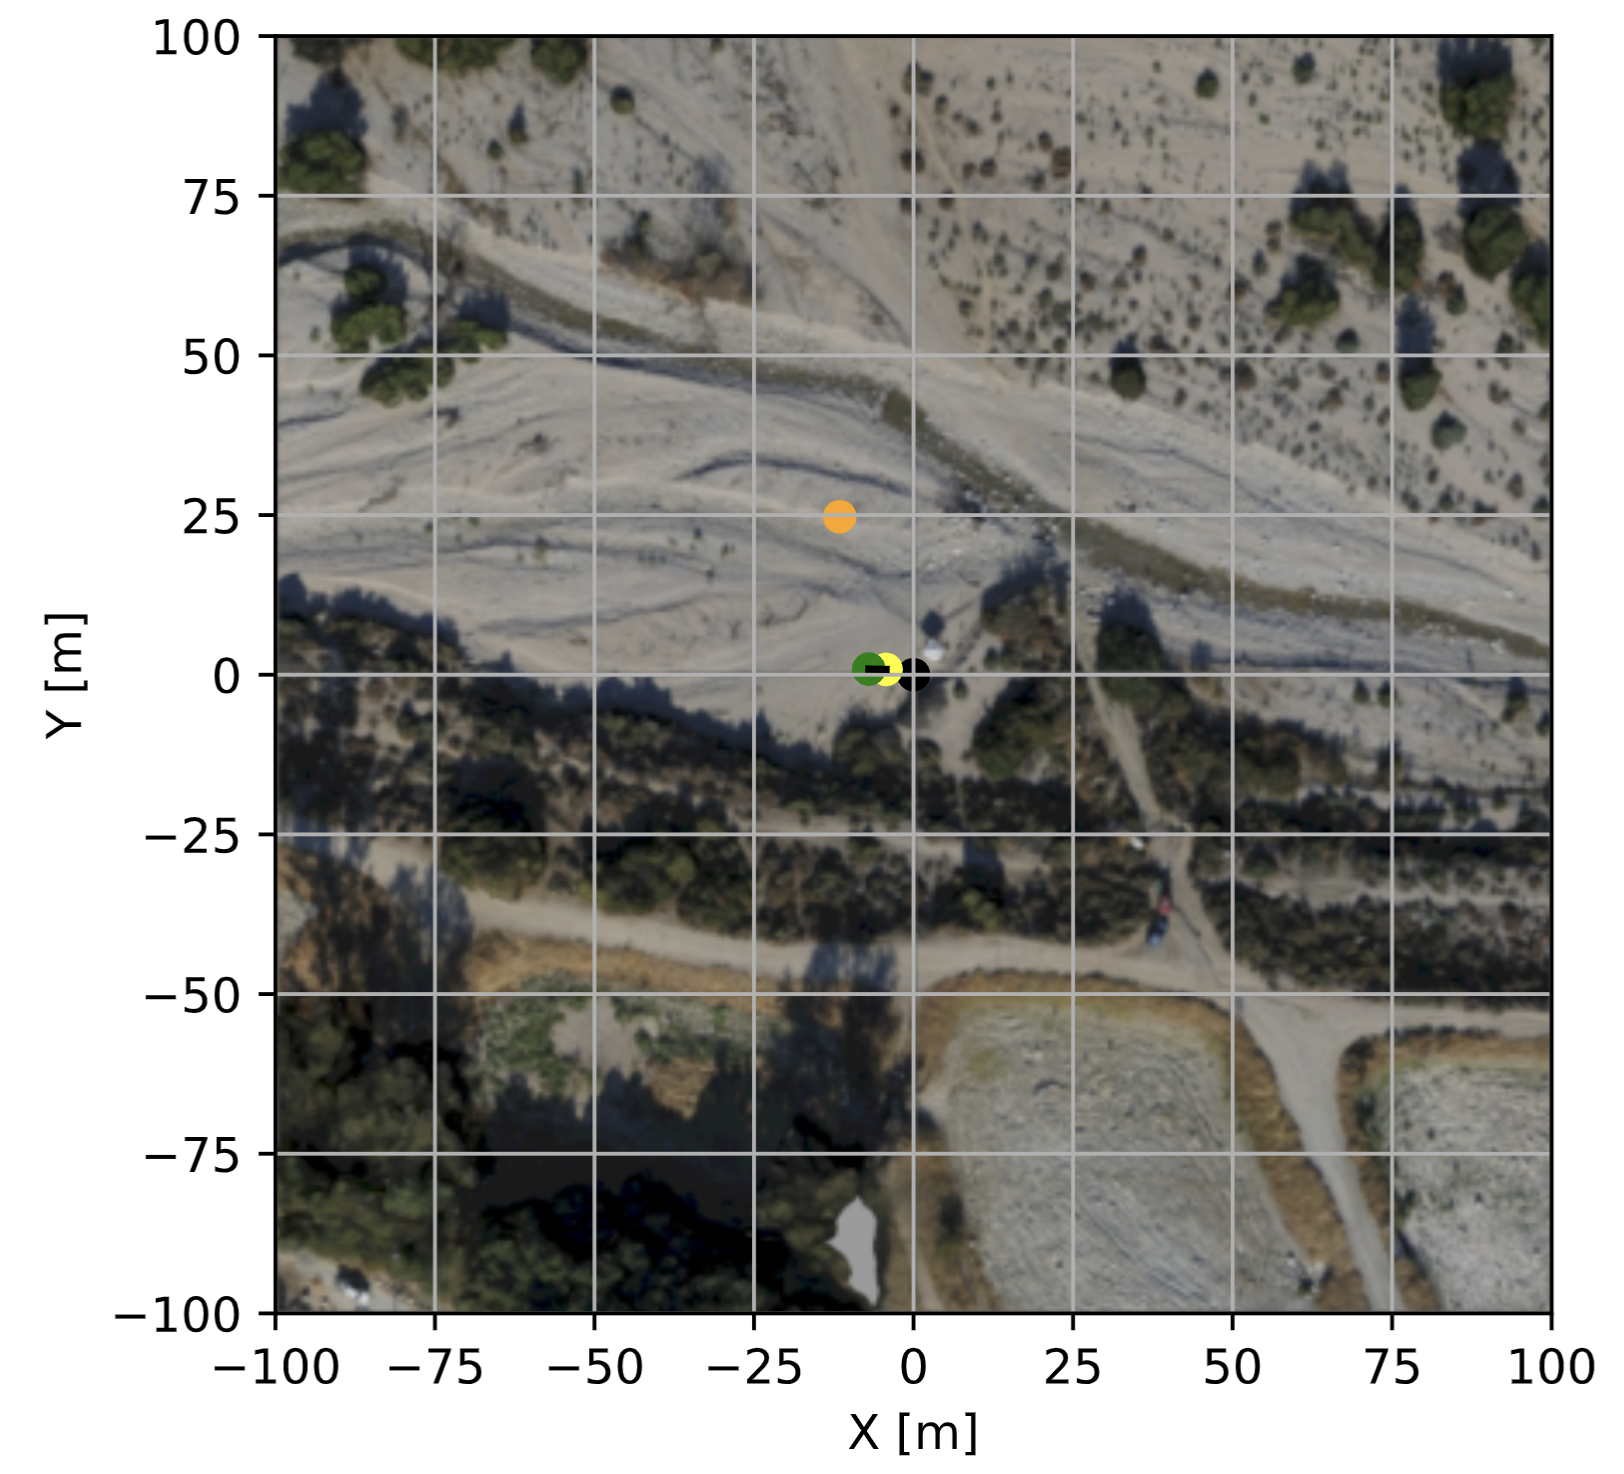
\includegraphics[scale=0.45]{images/appendix/run_analysis/demo_run.png}
\caption{Visual Analysis of demo landing: Black is the spawn of the drone, orange indicated the mission way point, yellow the first landing attempt which wasn't verified and green shows the final successful landing attempt.}
\label{fig:demo_run_landing}
\end{figure}
\subsection{Autonomy Log}

A summarizing log containing the most important information is shown below:

\begin{lstlisting}
    -----------------
    Iteration1:
    Spawn Randomization Disabled - Drone spawns at arroyo's \n
    default position: 0 0 0 0 0 3.5
    No additional landing sites spawned.
    Mission Waypoints added:
    Waypoint 0: (x: -24.739966478190148, y: -11.563968813290693, z: 100.0)
    --------
    Evaluation 1
    --------
    Run took 384.94275641441345s
    Landing Site Log:
    LS 1: [2024-04-21_23:44:43] [INFO]  Selecting Landing Site \n
    with ID 12 at (x: -0.834371, y: -4.30025, z: -0.4452)

    Landing Site Verification 1: Failure
    LS 2: [2024-04-21_23:47:26] [INFO]  Selecting Landing Site \n
    with ID 1834 at (x: -0.884371, y: -7.00025, z: -0.533367)

    Landing Site Verification 2: Successful
    Landing Sequence was initiated
    Checks:
    Rotation Check: Successful

    Conclusion: Success
    ---------------------------------
\end{lstlisting}

The entire autonomy log is displayed in the following:

\begin{lstlisting}
[2024-04-21_23:42:07] [INFO]  Estimated Time to execute Takeoff \n
and get to Flight Altitude! [Estimated Time: 41.000000 ]
[2024-04-21_23:42:07] [INFO]  State-Machine: \n
State transition table setup
[2024-04-21_23:42:07] [INFO]  Entering State Idle ...
[2024-04-21_23:42:07] [INFO]  State-Machine initialized
[2024-04-21_23:42:07] [INFO]  Initializing Autonomy
[2024-04-21_23:42:07] [INFO]  Waiting 12 seconds for \n 
System to boot ... 
[2024-04-21_23:42:19] [WARNING]  Failed to Set Parameter[MPC_Z_VEL_MAX_UP]
[2024-04-21_23:42:19] [WARNING]  Failed to Set Parameter[MPC_XY_CRUISE]
[2024-04-21_23:42:19] [WARNING]  Failed to Set Parameter[MPC_YAWRAUTO_MAX]
[2024-04-21_23:42:19] [WARNING]  Failed to Set Parameter[MPC_XY_VEL_ALL]
[2024-04-21_23:42:19] [INFO]  Initialized \n 
Navigation Parameters successfully!
[2024-04-21_23:42:19] [WARNING]  Error while \n 
Setting the Navigation Parameters!
[2024-04-21_23:42:19] [INFO]  Waiting 12 seconds for \n 
System to boot ... 
[2024-04-21_23:42:31] [INFO]  Initialized \n 
Navigation Parameters successfully!
[2024-04-21_23:42:31] [INFO]  [PX4] GPS activated!
[2024-04-21_23:42:31] [INFO]  [PX4] Height Reference set to GPS!
[2024-04-21_23:42:31] [INFO]  [PX4] External Vision deactivated!
[2024-04-21_23:42:32] [INFO]  System Initialized (with EKF2 GPS Parameters!
[2024-04-21_23:42:32] [INFO]  ROS Parameter Server updated!
[2024-04-21_23:42:32] [INFO]  Starting Autonomous Mission Execution!
[2024-04-21_23:42:32] [EVENT]:  Complete
[2024-04-21_23:42:32] [INFO]  Idle Behavior completed!
[2024-04-21_23:42:33] [EVENT]:  Complete
[2024-04-21_23:42:33] [INFO]  Exiting State Idle ...
[2024-04-21_23:42:33] [STATE TRANSITION]  State transition: Idle -> Init
[2024-04-21_23:42:33] [INFO]  Entering State Init ...
[2024-04-21_23:42:38] [INFO]  Start Pose: \n 
-0.277228, -0.0262564, -0.0260597, 0.0273177, -0.0170902, -3.04208
[2024-04-21_23:42:38] [INFO]  Initial Pose and Home Position saved!
[2024-04-21_23:42:38] [INFO]  Ready for GPS flights!
[2024-04-21_23:42:38] [INFO]  Successfully parsed CSV Mission File!
[2024-04-21_23:42:38] [WARNING]  Waypoints already in the \n 
Target Reference Frame! [ Reference Frame: LOCAL ]
[2024-04-21_23:42:38] [INFO]  Current Location x: -0.282364 y: -0.0325935
[2024-04-21_23:42:38] [INFO]  First Waypoint Location x: -24.74 y: -11.564
[2024-04-21_23:42:38] [INFO]  First Waypoint is 27.039729 meters away from \n 
the current position! Adding a new Waypoint at the current position!
[2024-04-21_23:42:38] [INFO]  Created Mission!
[2024-04-21_23:42:38] [INFO]  Mission Plan created!
[2024-04-21_23:42:38] [INFO]  Mission Plan ready to execute!
[2024-04-21_23:42:38] [INFO]  Estimator Interface is not used / disabled!
[2024-04-21_23:42:38] [INFO]  Skipped Initializing Healthguard!
[2024-04-21_23:42:38] [EVENT]:  Complete
[2024-04-21_23:42:38] [INFO]  Initialized System!
[2024-04-21_23:42:38] [EVENT]:  Complete
[2024-04-21_23:42:38] [INFO]  Exiting State Init ...
[2024-04-21_23:42:38] [STATE TRANSITION]  State transition: \n 
Init -> PreMissionChecks
[2024-04-21_23:42:38] [INFO]  Actuator Checks skipped! Ready to arm!
[2024-04-21_23:42:38] [INFO]  Battery check completed --> \n 
Ready for Mission!
[2024-04-21_23:42:38] [EVENT]:  Complete
[2024-04-21_23:42:38] [INFO]  Pre-Checks completed! \n 
Ready to arm!
[2024-04-21_23:42:38] [EVENT]:  Complete
[2024-04-21_23:42:38] [STATE TRANSITION]  State transition: \n 
PreMissionChecks -> Takeoff
[2024-04-21_23:42:38] [INFO]  Entering Takeoff State ...
[2024-04-21_23:42:38] [INFO]  Maximal Ascending Speed set to: 5.000000 !
[2024-04-21_23:42:38] [INFO]  Estimated Takeoff time is: 41.000000!
[2024-04-21_23:42:38] [WARNING]  Connected to the FCU!
[2024-04-21_23:42:38] [INFO]  Offboard Mode activated!
[2024-04-21_23:42:38] [INFO]  Arming completed!
[2024-04-21_23:42:38] [INFO]  Takeoff Action Started!
[2024-04-21_23:42:38] [WARNING]  Start Altitude is set to: -0.058790 m \n 
and the Takeoff Altitude is set to: 1.941210 m!
[2024-04-21_23:42:38] [INFO]  Takeoff Action Running ...
[2024-04-21_23:42:43] [INFO]  Takeoff Action Running ...
[2024-04-21_23:42:48] [INFO]  Takeoff Action Running ...
[2024-04-21_23:42:53] [INFO]  Takeoff Action Running ...
[2024-04-21_23:42:55] [INFO]  Takeoff Waypoint reached!
[2024-04-21_23:42:57] [INFO]  Hold Pose Action completed!
[2024-04-21_23:42:57] [EVENT]:  Complete
[2024-04-21_23:42:57] [INFO]  Takeoff altitude reached!
[2024-04-21_23:42:57] [EVENT]:  Complete
[2024-04-21_23:42:57] [STATE TRANSITION]  State transition: \n 
Takeoff -> Mission
[2024-04-21_23:42:57] [INFO]  Entering Mission State ...
[2024-04-21_23:42:57] [INFO]  Current Waypoint: 1 (Out of: 2)
[2024-04-21_23:42:57] [INFO]  Mission state was set to \n 
NavigateToWaypoint.
[2024-04-21_23:42:57] [INFO]  Mission initialized!
[2024-04-21_23:42:57] [INFO]  In total 2 waypoints to fly
[2024-04-21_23:44:06] [INFO]  Waypoint reached!
[2024-04-21_23:44:06] [INFO]  All current Waypoint-Actions completed!
[2024-04-21_23:44:06] [INFO]  Current Waypoint: 2 (Out of: 2)
[2024-04-21_23:44:06] [INFO]  Mission state was set to \n 
NavigateToWaypoint.
[2024-04-21_23:44:42] [INFO]  Waypoint reached!
[2024-04-21_23:44:42] [INFO]  Velocity set! (Setpoint: 2.000000 m/s))
[2024-04-21_23:44:43] [INFO]  Holding position finished!
[2024-04-21_23:44:43] [INFO]  All current Waypoint-Actions completed!
[2024-04-21_23:44:43] [INFO]  Mission Complete!
[2024-04-21_23:44:43] [EVENT]:  Complete
[2024-04-21_23:44:43] [INFO]  Mission Complete!
[2024-04-21_23:44:43] [EVENT]:  Complete
[2024-04-21_23:44:43] [INFO]  Exiting Mission State ...
[2024-04-21_23:44:43] [STATE TRANSITION]  State transition: \n 
Mission -> Land
[2024-04-21_23:44:43] [INFO]  Entering State_Land...
[2024-04-21_23:44:43] [INFO]  Initializing Landing Tree ...
[2024-04-21_23:44:43] [INFO]  Landing Tree initialized!
[2024-04-21_23:44:43] [INFO]  Check Landing Site Action
[2024-04-21_23:44:43] [INFO]  Landing Site List Check: \n 
larger than 0
[2024-04-21_23:44:43] [INFO]  GetLandingSiteAction
[2024-04-21_23:44:43] [INFO]  Getting Best landing sites \n 
at current location x: -25.013 y: -11.2604 z: 100.056
[2024-04-21_23:44:43] [INFO]  Loss of LS 12 at position \n 
x:-0.834371 y: -4.30025 z: -0.4452 loss: 0.864074, \n 
contrib size: -0.649404, contrib dist: 1.03603, \n 
contrib veralt: 0.0890372, contrib var: 0.000254673, \n 
contrib rough: 0.0498131
[2024-04-21_23:44:43] [INFO]  Loss of LS 42 at position \n 
x:-4.28437 y: -4.65025 z: -0.450161 loss: 0.983715, \n 
contrib size: -0.742495, contrib dist: 1.02834, \n 
contrib veralt: 1.00468, contrib var: 0.00103761, \n 
contrib rough: 0.0762918
[2024-04-21_23:44:43] [INFO]  Loss of LS 33 at position \n 
x:-3.98437 y: -8.75025 z: -0.580863 loss: 0.993144, \n 
contrib size: -0.371124, contrib dist: 1.02841, \n 
contrib veralt: 0.148057, contrib var: 0.000307739, \n 
contrib rough: 0.0574909
[2024-04-21_23:44:43] [INFO]  LSM: Landing Site has been selected
[2024-04-21_23:44:43] [INFO]  Selecting Landing Site with ID 12 at \n 
(x: -0.834371, y: -4.30025, z: -0.4452)
[2024-04-21_23:44:43] [INFO]  GetLandingSiteAction: \n 
Initial altitude was defined by current altitude which is 99.9901
[2024-04-21_23:44:43] [WARNING]  GetLandingSiteAction: \n 
Start altitude is above failsafe altitude - choosing start altitude.
[2024-04-21_23:44:43] [INFO]  Landing Site found!
[2024-04-21_23:44:43] [INFO]  AscendToClearAltitudeAction: \n 
Altitude reached!
[2024-04-21_23:44:43] [INFO]  RotateTowardsWaypointAction
[2024-04-21_23:44:43] [INFO]  NavigateTowardsWaypointAction
[2024-04-21_23:44:43] [INFO]  Successfully set velocity to navigate to \n 
waypoint with coordinates: x: -0.834371, y: -4.30025, z: 99.9901
[2024-04-21_23:45:22] [INFO]  Reached Pose with coordinates: \n 
x: -0.834371, y: -4.30025, z: 99.9901
[2024-04-21_23:45:22] [INFO]  ChangeAltitudeLSAction to 2.0548 which is \n 
2.5m above the landing site
[2024-04-21_23:47:11] [INFO]  ChangeAltitudeLSAction: \n 
Altitude reached!
[2024-04-21_23:47:26] [INFO]  Hold Pose Action completed!
[2024-04-21_23:47:26] [INFO]  Landing Site Verification Action at: \n 
2.14322 meters altitude
[2024-04-21_23:47:26] [WARNING]  Landing site verification failed at \n 
2.14322 meters. Verification altitude was: 8.90372 Resetting Landing site...
[2024-04-21_23:47:26] [WARNING]  Removing Landing Site with ID12
[2024-04-21_23:47:26] [WARNING]  Remaining IDs: \n 
589, 213, 206, 41, 217, 205, 52, 57, 45, 55, 59, 51, 204, \n 
49, 207, 202, 208, 203, 210, 1834, 
[2024-04-21_23:47:26] [INFO]  Check Landing Site Action
[2024-04-21_23:47:26] [INFO]  Landing Site List Check: larger than 0
[2024-04-21_23:47:26] [INFO]  GetLandingSiteAction
[2024-04-21_23:47:26] [INFO]  Getting Best landing sites at current location \n 
x: -2.05054 y: -2.97383 z: 2.13485
[2024-04-21_23:47:26] [INFO]  Loss of LS 1834 at position \n 
x:-0.884371 y: -7.00025 z: -0.533367 loss: -0.315955, \n 
contrib size: -0.798207, contrib dist: 0.0496904, \n 
contrib veralt: 0.0266822, contrib var: 0.000306336, \n 
contrib rough: 0.0359142
[2024-04-21_23:47:26] [INFO]  Loss of LS 589 at position \n 
x:-4.33437 y: -7.55025 z: -0.598968 loss: -0.119794, \n 
contrib size: -0.725, contrib dist: 0.0579942, \n 
contrib veralt: 0.657236, contrib var: 0.103212, \n 
contrib rough: 0.0608913
[2024-04-21_23:47:26] [INFO]  Loss of LS 206 at position \n 
x:-5.18437 y: -8.10025 z: -0.62499 loss: -0.0702529, \n 
contrib size: -0.65625, contrib dist: 0.0661194, \n 
contrib veralt: 0.657496, contrib var: 0.10416, \n 
contrib rough: 0.0218446
[2024-04-21_23:47:26] [INFO]  LSM: Landing Site has been selected
[2024-04-21_23:47:26] [INFO]  Selecting Landing Site with ID 1834 at \n 
(x: -0.884371, y: -7.00025, z: -0.533367)
[2024-04-21_23:47:26] [INFO]  GetLandingSiteAction: \n 
Initial altitude was defined by highest detected obstacle at 2.73586
[2024-04-21_23:47:26] [INFO]  XY-Distance based interpolation yielded \n 
clearing altitude of 8.93774
[2024-04-21_23:47:26] [INFO]  Landing Site found!
[2024-04-21_23:47:51] [INFO]  AscendToClearAltitudeAction: \n 
Altitude reached!
[2024-04-21_23:47:51] [INFO]  RotateTowardsWaypointAction
[2024-04-21_23:47:51] [INFO]  NavigateTowardsWaypointAction
[2024-04-21_23:47:51] [INFO]  Successfully set velocity \n 
to navigate to waypoint with coordinates: \n 
x: -0.884371, y: -7.00025, z: 8.93774
[2024-04-21_23:48:20] [INFO]  Reached Pose with coordinates: \n 
x: -0.884371, y: -7.00025, z: 8.93774
[2024-04-21_23:48:20] [INFO]  ChangeAltitudeLSAction \n 
to 1.96775 which is 2.5m above the landing site
[2024-04-21_23:48:32] [INFO]  ChangeAltitudeLSAction: \n 
Altitude reached!
[2024-04-21_23:48:47] [INFO]  Hold Pose Action completed!
[2024-04-21_23:48:47] [INFO]  Landing Site Verification Action at: \n 
2.22133 meters altitude
[2024-04-21_23:48:47] [INFO]  Landing site was verified at \n 
2.75358 meters off the ground
[2024-04-21_23:48:47] [INFO]  Landing  at \n 
(-0.584371, -7.50025, -0.53225)
[2024-04-21_23:48:47] [INFO]  Landing Site Location Updated!
[2024-04-21_23:48:47] [INFO]  NavigateTowardsWaypointAction
[2024-04-21_23:48:47] [INFO]  Successfully set velocity to \n 
navigate to waypoint with coordinates: \n 
x: -0.584371, y: -7.50025, z: 2.22133
[2024-04-21_23:48:51] [INFO]  Reached Pose with coordinates: \n 
x: -0.584371, y: -7.50025, z: 2.22133
[2024-04-21_23:48:51] [INFO]  Landing Action: \n 
Landing at Z of detected landing site.
[2024-04-21_23:48:54] [INFO]  Landing ...
[2024-04-21_23:48:57] [INFO]  Landing ...
[2024-04-21_23:49:00] [INFO]  Landing ...
[2024-04-21_23:49:03] [INFO]  Landing ...
[2024-04-21_23:49:06] [INFO]  Landing ...
[2024-04-21_23:49:06] [INFO]  Landing detected!
[2024-04-21_23:49:06] [INFO]  Disarmed!
[2024-04-21_23:49:06] [EVENT]:  Complete
[2024-04-21_23:49:06] [INFO]  Landing Behavior completed!
[2024-04-21_23:49:06] [EVENT]:  Complete
[2024-04-21_23:49:06] [STATE TRANSITION]  \n 
State transition: Land -> Terminate
[2024-04-21_23:49:06] [INFO]  Vehicle is landed!

\end{lstlisting}

\subsection{Flight Controller Connection Loss}
Lastly, hereafter I show a run which lost connection to the flight controller mid-flight:

\begin{lstlisting}
[2024-04-23_22:00:08] [INFO]  State-Machine: \n 
State transition table setup
[2024-04-23_22:00:08] [INFO]  Entering State Idle ...
[2024-04-23_22:00:08] [INFO]  State-Machine initialized
[2024-04-23_22:00:08] [INFO]  Initializing Autonomy
[2024-04-23_22:00:08] [INFO]  Waiting 12 seconds for System to boot ... 
[2024-04-23_22:00:20] [WARNING]  Failed to Set \n 
Parameter[MPC_Z_VEL_MAX_UP]
[2024-04-23_22:00:20] [WARNING]  Failed to Set \n 
Parameter[MPC_XY_CRUISE]
[2024-04-23_22:00:20] [WARNING]  Failed to Set \n 
Parameter[MPC_YAWRAUTO_MAX]
[2024-04-23_22:00:20] [WARNING]  Failed to Set \n 
Parameter[MPC_XY_VEL_ALL]
[2024-04-23_22:00:20] [INFO]  Initialized \n 
Navigation Parameters successfully!
[2024-04-23_22:00:20] [WARNING]  Error while Setting \n 
the Navigation Parameters!
[2024-04-23_22:00:20] [INFO]  Waiting 12 seconds for \n 
System to boot ... 
[2024-04-23_22:00:32] [INFO]  Initialized \n 
Navigation Parameters successfully!
[2024-04-23_22:00:32] [INFO]  [PX4] GPS activated!
[2024-04-23_22:00:32] [INFO]  [PX4] Height Reference set to GPS!
[2024-04-23_22:00:32] [INFO]  [PX4] External Vision deactivated!
[2024-04-23_22:00:33] [INFO]  System Initialized (with EKF2 GPS Parameters!
[2024-04-23_22:00:33] [INFO]  ROS Parameter Server updated!
[2024-04-23_22:00:33] [INFO]  Starting Autonomous \n 
Mission Execution!
[2024-04-23_22:00:34] [EVENT]:  Complete
[2024-04-23_22:00:34] [INFO]  Idle Behavior completed!
[2024-04-23_22:00:34] [EVENT]:  Complete
[2024-04-23_22:00:34] [INFO]  Exiting State Idle ...
[2024-04-23_22:00:34] [STATE TRANSITION]  State transition: \n 
Idle -> Init
[2024-04-23_22:00:34] [INFO]  Entering State Init ...
[2024-04-23_22:00:39] [INFO]  Start Pose: \n 
59.4398, 32.3157, 39.8456, 0.00186781, -9.09566e-05, -0.00994173
[2024-04-23_22:00:39] [INFO]  Initial Pose and \n 
Home Position saved!
[2024-04-23_22:00:39] [INFO]  Ready for GPS flights!
[2024-04-23_22:00:39] [INFO]  Successfully parsed CSV Mission File!
[2024-04-23_22:00:39] [WARNING]  Waypoints already in the \n 
Target Reference Frame! [ Reference Frame: LOCAL ]
[2024-04-23_22:00:39] [INFO]  Current Location \n 
x: 59.4394 y: 32.3134
[2024-04-23_22:00:39] [INFO]  First Waypoint Location \n 
x: -12.7774 y: -19.8106
[2024-04-23_22:00:39] [INFO]  First Waypoint is \n 
89.062746 meters away from the current position! \n 
Adding a new Waypoint at the current position!
[2024-04-23_22:00:39] [INFO]  Created Mission!
[2024-04-23_22:00:39] [INFO]  Mission Plan created!
[2024-04-23_22:00:39] [INFO]  Mission Plan ready to execute!
[2024-04-23_22:00:39] [INFO]  Estimator Interface is not used / disabled!
[2024-04-23_22:00:39] [INFO]  Skipped Initializing Healthguard!
[2024-04-23_22:00:39] [EVENT]:  Complete
[2024-04-23_22:00:39] [INFO]  Initialized System!
[2024-04-23_22:00:39] [EVENT]:  Complete
[2024-04-23_22:00:39] [INFO]  Exiting State Init ...
[2024-04-23_22:00:39] [STATE TRANSITION]  State transition: \n 
Init -> PreMissionChecks
[2024-04-23_22:00:39] [INFO]  Actuator Checks skipped! \n 
Ready to arm!
[2024-04-23_22:00:39] [INFO]  Battery check completed --> \n 
Ready for Mission!
[2024-04-23_22:00:39] [EVENT]:  Complete
[2024-04-23_22:00:39] [INFO]  Pre-Checks completed! \n 
Ready to arm!
[2024-04-23_22:00:39] [EVENT]:  Complete
[2024-04-23_22:00:39] [STATE TRANSITION]  State transition: \n 
PreMissionChecks -> Takeoff
[2024-04-23_22:00:39] [INFO]  Entering Takeoff State ...
[2024-04-23_22:00:39] [INFO]  Maximal Ascending Speed set to: 5.000000 !
[2024-04-23_22:00:39] [INFO]  Estimated Takeoff time is: 41.000000!
[2024-04-23_22:00:39] [WARNING]  Connected to the FCU!
[2024-04-23_22:00:39] [INFO]  Offboard Mode activated!
[2024-04-23_22:00:39] [INFO]  Arming completed!
[2024-04-23_22:00:39] [INFO]  Takeoff Action Started!
[2024-04-23_22:00:39] [WARNING]  Start Altitude is set to: \n 
39.860235 m and the Takeoff Altitude is set to: 41.860235 m!
[2024-04-23_22:00:39] [INFO]  Takeoff Action Running ...
[2024-04-23_22:00:44] [INFO]  Takeoff Action Running ...
[2024-04-23_22:00:49] [INFO]  Takeoff Action Running ...
[2024-04-23_22:00:54] [INFO]  Takeoff Action Running ...
[2024-04-23_22:00:59] [INFO]  Takeoff Action Running ...
[2024-04-23_22:01:04] [INFO]  Takeoff Action Running ...
[2024-04-23_22:01:08] [INFO]  Takeoff Waypoint reached!
[2024-04-23_22:01:10] [INFO]  Hold Pose Action completed!
[2024-04-23_22:01:10] [EVENT]:  Complete
[2024-04-23_22:01:10] [INFO]  Takeoff altitude reached!
[2024-04-23_22:01:10] [EVENT]:  Complete
[2024-04-23_22:01:10] [STATE TRANSITION]  State transition: \n 
Takeoff -> Mission
[2024-04-23_22:01:10] [INFO]  Entering Mission State ...
[2024-04-23_22:01:10] [INFO]  Current Waypoint: 1 (Out of: 2)
[2024-04-23_22:01:10] [INFO]  Mission state was set to \n 
NavigateToWaypoint.
[2024-04-23_22:01:10] [INFO]  Mission initialized!
[2024-04-23_22:01:10] [INFO]  In total 2 waypoints to fly
[2024-04-23_22:01:53] [INFO]  Waypoint reached!
[2024-04-23_22:01:53] [INFO]  All current Waypoint-Actions completed!
[2024-04-23_22:01:53] [INFO]  Current Waypoint: 2 (Out of: 2)
[2024-04-23_22:01:53] [INFO]  Mission state was set to \n 
NavigateToWaypoint.
[2024-04-23_22:03:24] [INFO]  Waypoint reached!
[2024-04-23_22:03:24] [INFO]  Velocity set! (Setpoint: 2.000000 m/s))
[2024-04-23_22:03:25] [INFO]  Holding position finished!
[2024-04-23_22:03:25] [INFO]  All current Waypoint-Actions completed!
[2024-04-23_22:03:25] [INFO]  Mission Complete!
[2024-04-23_22:03:25] [EVENT]:  Complete
[2024-04-23_22:03:25] [INFO]  Mission Complete!
[2024-04-23_22:03:25] [EVENT]:  Complete
[2024-04-23_22:03:25] [INFO]  Exiting Mission State ...
[2024-04-23_22:03:25] [STATE TRANSITION]  State transition: \n 
Mission -> Land
[2024-04-23_22:03:25] [INFO]  Entering State_Land...
[2024-04-23_22:03:25] [INFO]  Initializing Landing Tree ...
[2024-04-23_22:03:25] [INFO]  Landing Tree initialized!
[2024-04-23_22:03:25] [INFO]  Check Landing Site Action
[2024-04-23_22:03:25] [INFO]  Landing Site List Check: \n 
larger than 0
[2024-04-23_22:03:25] [INFO]  GetLandingSiteAction
[2024-04-23_22:03:26] [INFO]  Getting Best landing sites at current location \n 
x: -12.5608 y: -19.6724 z: 99.9481
[2024-04-23_22:03:26] [INFO]  Loss of LS 499 at position \n 
x:-0.470386 y: -12.2437 z: -0.597542 loss: 0.916079, \n 
contrib size: -0.997011, contrib dist: 1.01542, \n 
contrib veralt: 1.00566, contrib var: 0.189603, \n 
contrib rough: 0.0114712
[2024-04-23_22:03:26] [INFO]  Loss of LS 58 at position \n 
x:27.3796 y: -1.14372 z: 3.56173 loss: 1.38689, \n 
contrib size: -0.192888, contrib dist: 1.05966, \n 
contrib veralt: 0.964176, contrib var: 0.139055, \n 
contrib rough: 0.0408271
[2024-04-23_22:03:26] [INFO]  Loss of LS 39 at position \n 
x:28.0296 y: -0.293723 z: 3.59092 loss: 1.40956, \n 
contrib size: -0.110222, contrib dist: 1.06338, \n 
contrib veralt: 0.963344, contrib var: 0.140886, \n 
contrib rough: 0.0481275
[2024-04-23_22:03:26] [INFO]  LSM: Landing Site has been selected
[2024-04-23_22:03:26] [INFO]  Selecting Landing Site with ID 499 at \n 
(x: -0.470386, y: -12.2437, z: -0.597542)
[2024-04-23_22:03:26] [INFO]  GetLandingSiteAction: \n 
Initial altitude was defined by current altitude which is 99.924
[2024-04-23_22:03:26] [WARNING]  GetLandingSiteAction: \n 
Start altitude is above failsafe altitude - choosing start altitude.
[2024-04-23_22:03:26] [INFO]  Landing Site found!
[2024-04-23_22:03:26] [INFO]  AscendToClearAltitudeAction: \n 
Altitude reached!
[2024-04-23_22:03:26] [INFO]  RotateTowardsWaypointAction
[2024-04-23_22:03:26] [INFO]  NavigateTowardsWaypointAction
[2024-04-23_22:03:26] [INFO]  Successfully set velocity to \n 
navigate to waypoint with coordinates: x: -0.470386, y: -12.2437, z: 99.924
[2024-04-23_22:03:43] [INFO]  Reached Pose with coordinates: \n 
x: -0.470386, y: -12.2437, z: 99.924
[2024-04-23_22:03:43] [INFO]  ChangeAltitudeLSAction to \n 
1.87749 which is 2.5m above the landing site

\end{lstlisting}

As can be seen, the flight controller connection was lost shortly after the descent to the verification altitude was commenced.

